\documentclass{article}
\usepackage{graphicx}
\usepackage[T1]{fontenc}
% LTeX: language=es,eng
\usepackage[spanish]{babel}
\graphicspath{ {./resources/} }
\usepackage{float}

\begin{document}

\section{Introducción}

La siguiente guía de instalación busca guiar al usuario en la configuración básica de un laboratorio de Oracle Real Application Clusters, esta guía no busca enseñarle al usuario a utilizar Linux, pero si buscara proporcionar un poco de contexto adicional sobre ciertos comandos de Unix. El laboratorio utiliza 3 máquinas virtuales, las cuales usaran Linux con distribuciones basadas en Ubuntu y RHEL, por otro lado el sistema operativo puede ser cualquiera de preferencia por el usuario, pero en este caso se usará Pop\_Os!, el cual se encuentra basado en Ubuntu.

\section{Configuración de Máquinas Virtuales}

El primer paso consiste en preparar nuestras máquinas virtuales para los nodos de Oracle DB, estos usarán Oracle Linux 7 con Oracle DB 19c, acá cada nodo tiene cuenta con los siguientes requerimientos.

\begin{itemize}
    \item 4 GB de memoria RAM.
    \item 100 GB de almacenamiento físico.
    \item 2 núcleos de procesamiento.
\end{itemize}

Empezando con la creación del primer nodo en este cluster lo llamaremos "node1", aparte de las especificaciones ya mencionadas es necesario crear 3 adaptadores de red:

\begin{itemize}
    \item Host-only Adapter: Usado para conectar a la base de datos hacia otros aplicativos. 
    \item Internal Network Adapter: Usado por la red interna del clúster. 
    \item Bridged Adapter: Usado para conectarse hacia el internet, usando al sistema operativo huésped. 
\end{itemize}

\begin{figure}[H]
    \begin{center}
        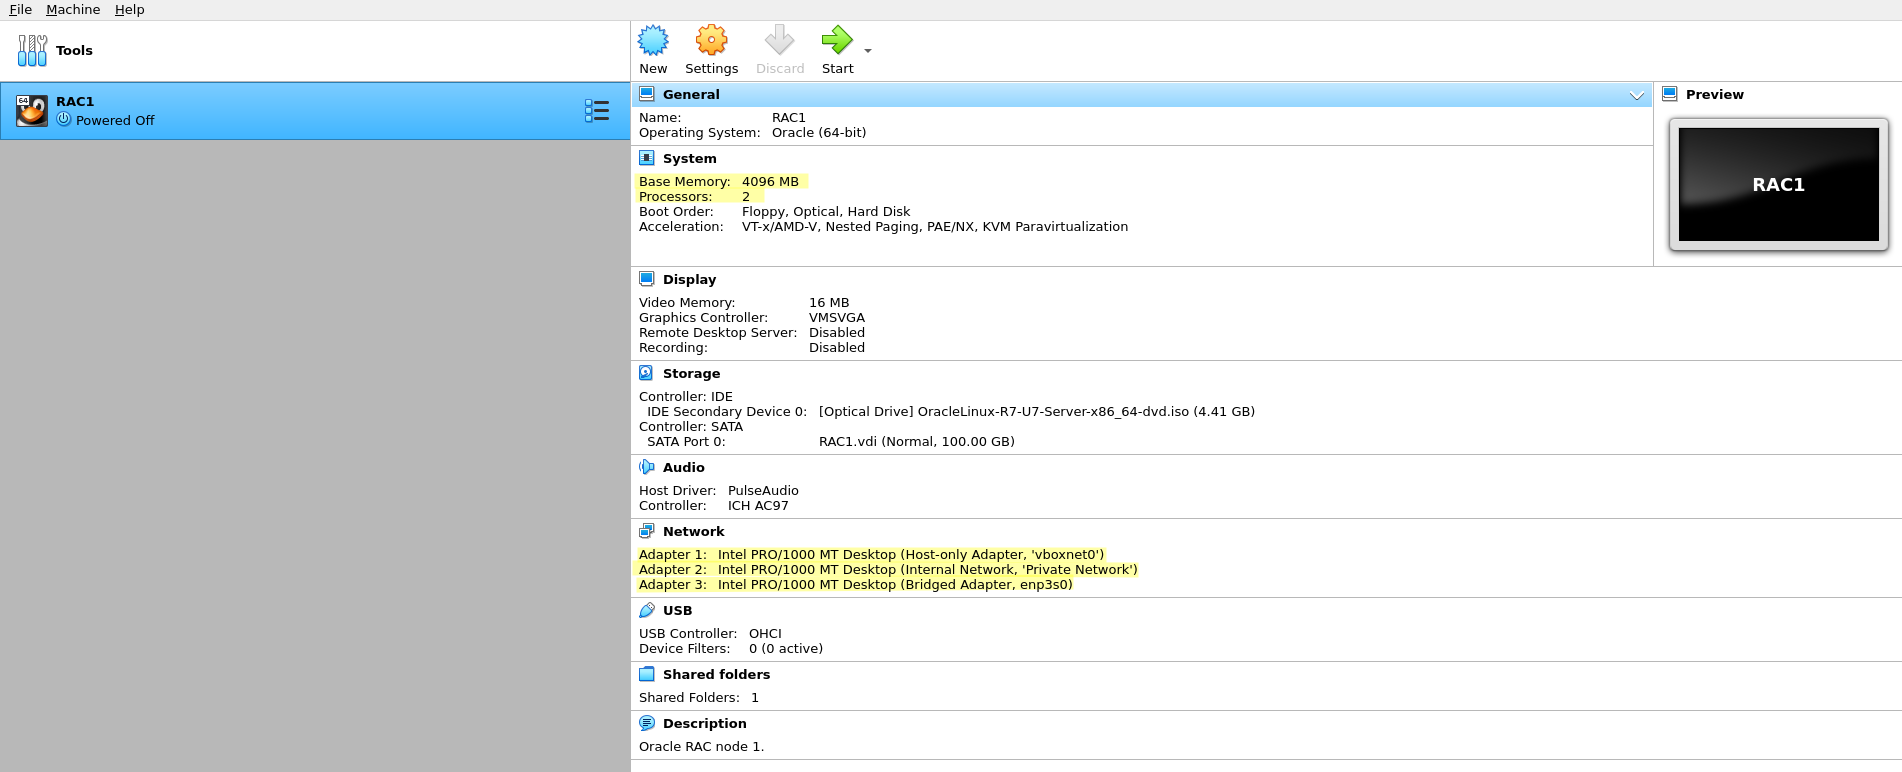
\includegraphics[width=0.95\textwidth]{vm_base.png}
    \end{center}
    \caption{Pantalla de inicio de Configuración de la Máquina Virtual}
\end{figure}

Al momento de iniciar la máquina virtual e insertar el archivo ISO con Oracle Linux 7, podemos empezar a configurar la instalación del sistema operativo. Acá iniciaremos con la configuración de partición del disco desde aca se selecciona "Installation Destination", en donde se puede ver el disco creado y las opciones de particiones, aca se selecionara "I will configure Partitioning".

\end{document}
